\section{代码组织}

\subsection{代码目录结构}

\href{https://github.com/occlum/sworndisk-linux-rs}{sworndisk-linux-rs} 仓库包含 \href{https://github.com/Rust-for-Linux/linux}{rust-for-linux} 的完整代码和 \href{https://github.com/occlum/sworndisk-linux-rs/tree/rust/modules/sworndisk}{SwornDisk 内核模块}代码,后者位于 modules/sworndisk 目录下:

\begin{minted}{shell}
  |- .cargo
  |   |- config.toml     # 项目 Cargo 配置文件,主要指定了使用 rustc 时需要附加的编译参数
  |- deps                # 项目依赖的 crates 目录
  |   |- cmwq            # Linux 工作队列 (CMWQ) 封装
  |   |- crypto          # Linux 内核加密 API 封装
  |   |- device-mapper   # Linux 块 I/O  (bio) 与 Device Mapper 框架封装
  |- dm-sworndisk        # SwornDisk Device Mapper 内核模块源码目录
  |   |- Cargo.toml
  |   |- src
  |       |- constant.rs      # 定义 SwornDisk 常量,如块、段大小等
  |       |- context.rs       # 定义用于储存 SwornDisk 上下文的结构,如各个段的实例
  |       |- handler.rs       # 定义处理 Device Mapper 事件 (ctr, dtr, map) 的方法
  |       |- lib.rs           # SwornDisk 内核模块入口 (entry)
  |       |- prelude.rs
  |       |- regions              # 磁盘布局区域实现
  |       |   |- checkpoint       # Checkpoint 区域
  |       |   |   |- bitc.rs      # BIT Category
  |       |   |   |- dst.rs       # Data Segment Table
  |       |   |   |- mod.rs     
  |       |   |   |- svt.rs       # Segment Validity Table
  |       |   |- data             # 数据段区域
  |       |   |   |- mod.rs
  |       |   |   |- segment.rs
  |       |   |- index            # 索引段区域
  |       |   |   |- bit.rs       # Block Index Table (BIT) 实现
  |       |   |   |- memtable.rs  # MemTable 实现
  |       |   |   |- mod.rs
  |       |   |   |- record.rs    # Record 结构
  |       |   |   |- segment.rs   # 索引段结构实现
  |       |   |- mod.rs
  |       |   |- superblock.rs    # 超级块
  |       |- types.rs         # 类型定义
  |       |- unittest.rs      # 单元测试
  |       |- utils            # 数据结构和工具函数
  |       |   |- bitmap.rs          # BitMap
  |       |   |- debug_ignore.rs    # debug_ignore crate 实现
  |       |   |- linked_list.rs     # Rust LinkedList 实现
  |       |   |- lru.rs             # LRU 缓存实现
  |       |   |- mod.rs
  |       |   |- traits.rs          # 需要的 traits 定义 (Serialize, Deserialze..)
  |       |- workers
  |           |- compaction.rs      # Major Compaction 逻辑
  |           |- io.rs              # 处理 I/O 请求
  |           |- mod.rs
  |-- Kbuild
  |-- Makefile
  |-- README.md
  |-- scripts
      |-- fio.conf            # fio 性能测试配置文件
      |-- generate_cmd.sh     # 生成编译时所需的 cmd 文件
      |-- insmod.sh           # 加载内核模块、创建 SwornDisk 示例命令
      |-- restore.sh          # 卸载内核模块、卸载 SwornDisk 示例命令
\end{minted}

\subsection{rust-for-linux}

\subsubsection{原理}

\begin{figure}[H]
  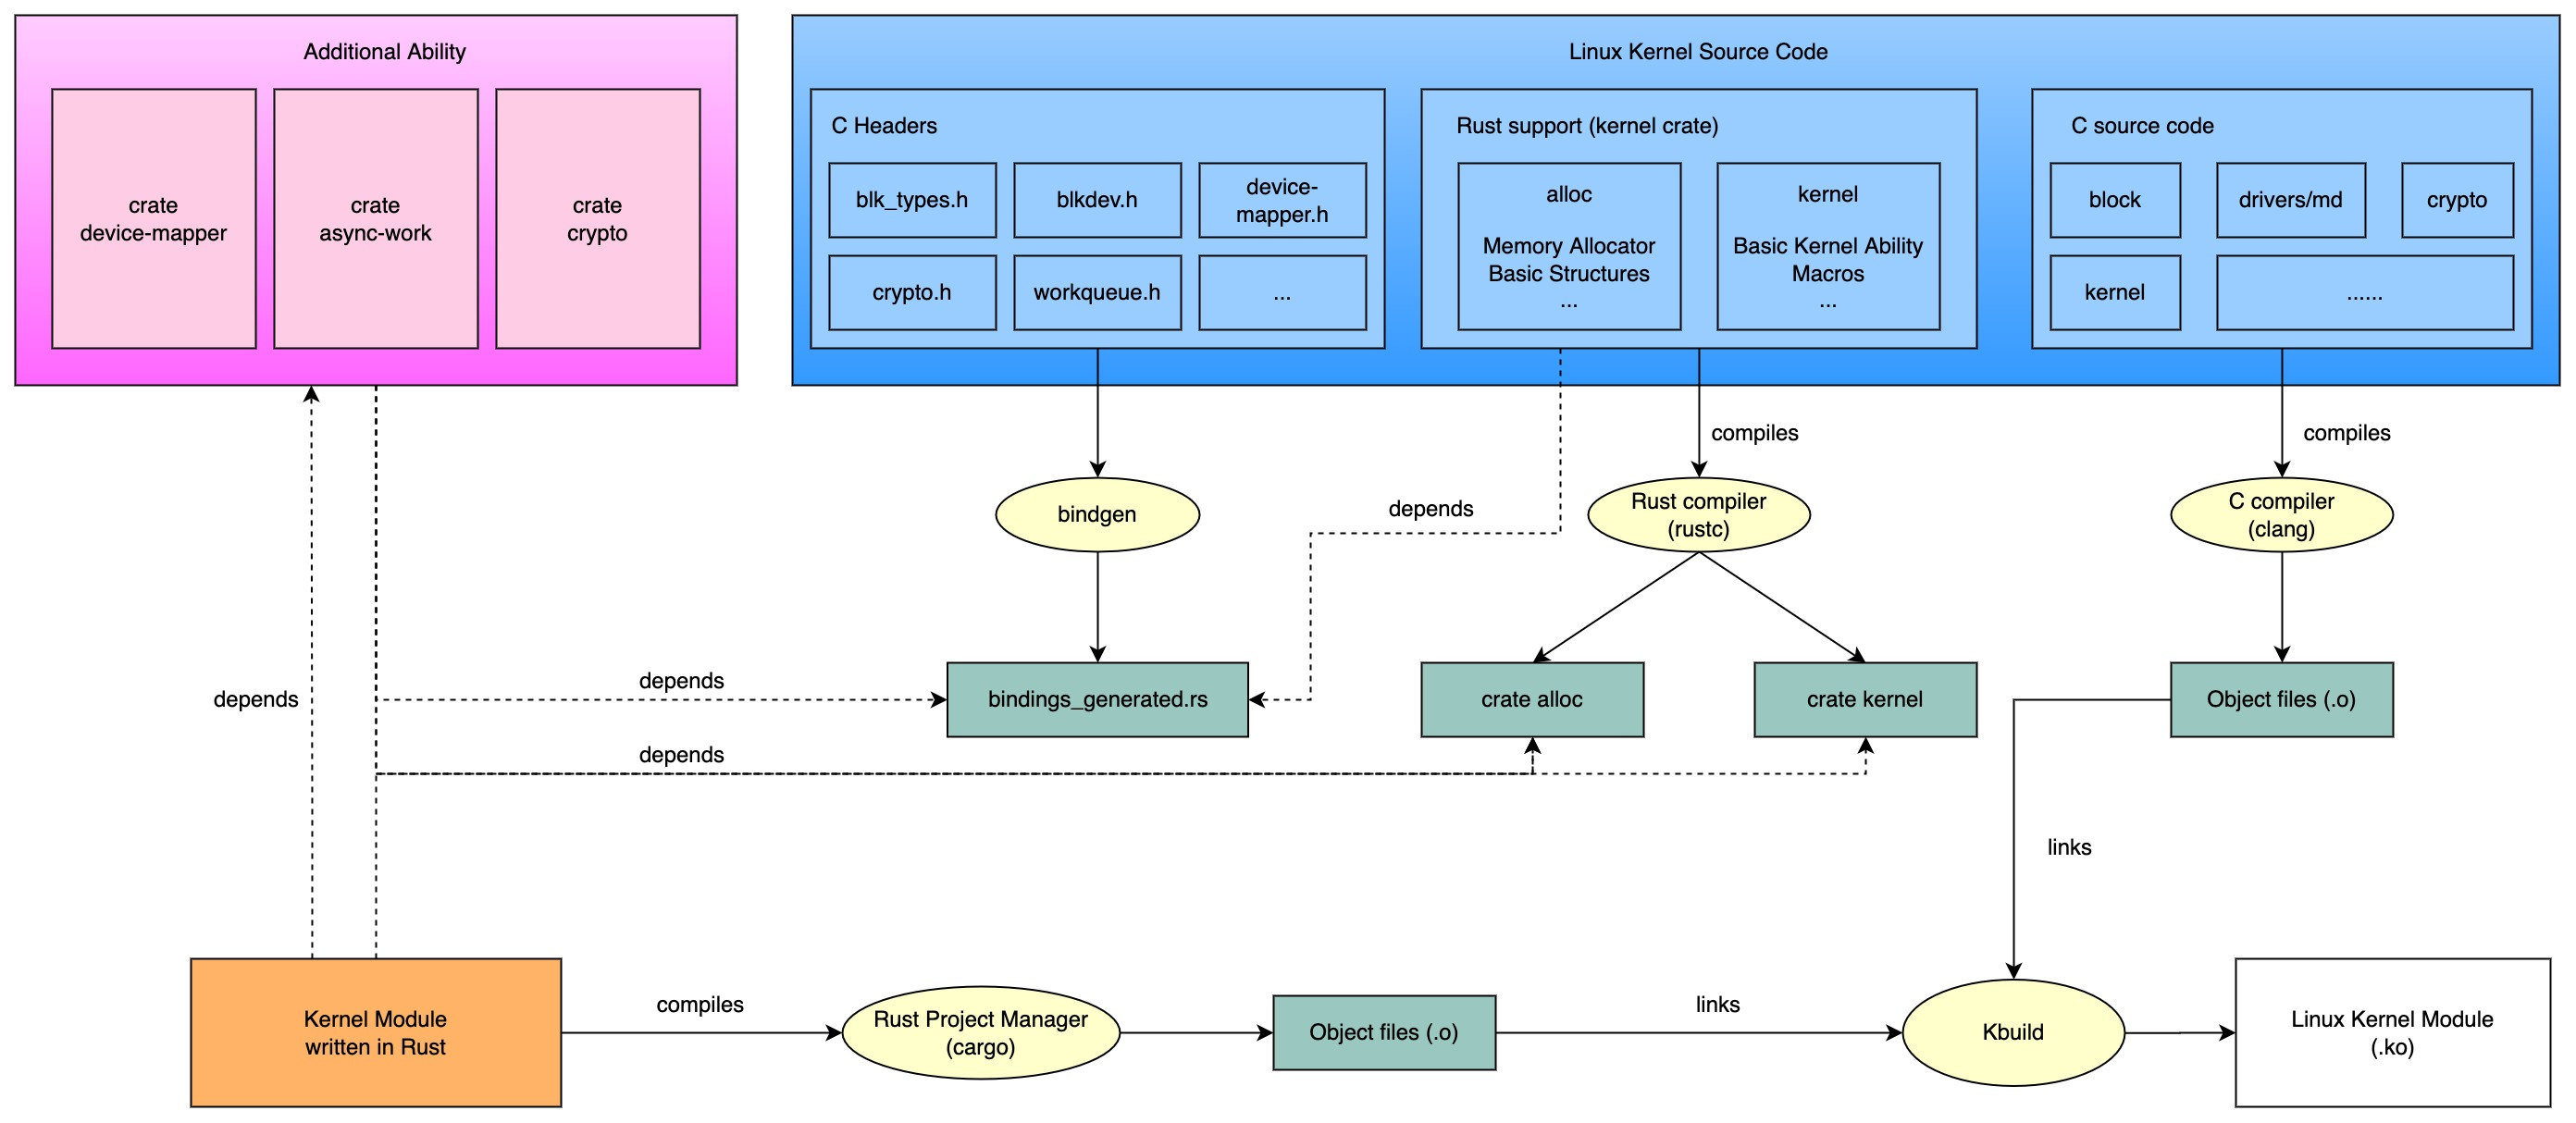
\includegraphics[width=\textwidth]{images/rust-for-linux-ability.jpg}
  \caption{基于 rust-for-linux 编写内核模块的原理图}
  \label{rust-for-linux-kernel-module-theory}
\end{figure}

图 \ref{rust-for-linux-kernel-module-theory} 展示了:

\begin{itemize}
  \item \textbf{rust-for-linux 项目提供 Rust 支持的方式}
  \begin{itemize}
    \item 首先,该项目提供了一套工具链 (rustc, bindgen, ...),并在内核的 Makefile 中定义了如何编译、链接与处理 Rust 源代码。
    \item 在内核的源码树中加入了 Rust 语言的核心能力 (alloc, core),并通过一个 \mintinline{text}{helper.h} 引入需要的 Linux 内核头文件,利用 bindgen 生成 \mintinline{text}{bindings_generated.rs} 文件。
    \item \mintinline{text}{bindings_generated.rs} 文件包含与上述头文件定义的 C 函数签名对应的 Rust 函数(除宏定义和 inline 函数,如果要在 Rust 中使用宏或 inline 函数则需要通过重新定义一个代理 \mintinline{text}{rust_helper_...} 来实现)。
    \item 根据 bindings 封装了一套使用 Linux 部分内核能力的 crate:\mintinline{text}{kernel},封装了如红黑树、互斥锁等 Linux 内核功能。
  \end{itemize}

  \item \textbf{向 rust-for-linux 拓展功能的方式}
  \begin{itemize}
    \item 第一种方法是直接向 \mintinline{text}{kernel} crate 添加内容。在 out-of-tree 的内核模块中,可以直接使用 kernel crate 中的内容。
    \item 第二种方法是将需要添加的内容独立成一个 crate,通过 Rust 的 extern crate 声明对 alloc, core, kernel 的依赖,然后在使用 rustc 编译时添加链接参数 \mintinline{text}{-L/path/to/xxx.o} 链接 alloc, core, kernel 等 crate.
  \end{itemize}

  \item \textbf{使用 Rust 编写内核模块的流程} \quad 根据 rust-for-linux 的 Makefile 中提供的对 .rs 文件的处理方式,分别经过 rustc 编译、ld.lld 链接,经过 modpost, lto 等一系列操作产生 .ko 格式的内核模块。
\end{itemize}

\subsubsection{在 rust-for-linux 上做出的改动}

尽管 SwornDisk 对 rust-for-linux 项目添加的能力 (Device Mapper 等) 都通过独立于内核代码的 crate 形式实现,但由于 rust-for-linux 本身在 API 设计上有一些问题无法满足我们的需求,因此对 rust-for-linux 项目本身也有少量的修改,包括:

\begin{itemize}
  \item 在 \mintinline{text}{rust/kernel/bindings_helper.h} 中添加了所需要的内核 C API 所在的头文件引用。
  \item 在 \mintinline{text}{rust/kernel/lib.rs} 中,修改了 \mintinline{rust}{ThisModule} 的成员可见性为 \mintinline{rust}{pub}。
  \item 在 \mintinline{text}{rust/helpers.c} 中添加了一些 inline 函数或宏的 binding 函数,以 \mintinline{c}{rust_helper_<function_name>} 的形式给出。
  \item 修改了 \mintinline{text}{Makefile} 和 \mintinline{text}{scripts/Makefile.build} 中与 Rust 编译相关的部分,主要是添加或去除了某些参数。
\end{itemize}


\subsubsection{基于 rust-for-linux 添加的内容}

为了实现 SwornDisk,我们主要补充了关于块 I/O, Device Mapper, 内核加密 API 和内核工作队列 CMWQ 的支持。

\begin{table}[H]
  \caption{Rust 容器与 C 结构体对应关系表}
  \begin{center}
  \begin{tabular}{ccc}
  \toprule
  C 结构                              & 对应 Rust 容器                  & 作用              \\
  \midrule
  \textit{struct block\_device}       & \textit{device\_mapper::BlockDevice}   & 表示块设备信息       \\ 
  \textit{struct bio}                 & \textit{device\_mapper::Bio}           &  表示块 I/O 请求信息 \\ 
  \textit{struct target\_type}        & \textit{device\_mapper::TargetType}  & 表示 Device Mapper 目标设备类型信息         \\ 
  \textit{struct dm\_dev}             & \textit{device\_mapper::DmDev}       & 表示 Device Mapper 映射的虚拟设备         \\ 
  \textit{struct dm\_target}          & \textit{device\_mapper::DmTarget}    & 表示 Device Mapper 目标设备实例         \\ 
  \textit{struct dm\_block\_manager}  & \textit{device\_mapperDmBlockManager}       & \multirow{2}{*}{用于 Device Mapper 中块设备的读写} \\ 
  \textit{struct dm\_block}           & \textit{device\_mapperDmBlock}              &                                       \\ 
  \textit{struct dm\_io\_region}      & \textit{device\_mapper::DmIoClient}       &                                       \\ 
  \textit{struct dm\_io\_request}     & \textit{device\_mapper::DmIoRequest}      &                                       \\ 
  \hline
  \textit{struct crypto\_aead}        & \textit{crypto::Aead}         & AEAD 加密实例 \\ 
  \textit{struct aead\_request}       & \textit{crypto::AeadRequest}  & AEAD 加密请求 \\ 
  \textit{struct scatterlist}         & \textit{crypto::ScatterList}  & Linux 散列表 \\ 
  \hline
  \textit{struct workqueue\_struct}   & \textit{cmwq::WorkQueue}   & CMWQ 工作队列 \\ 
  \textit{struct work\_struct}        & \textit{cmwq::WorkStruct}  & CMWQ 工作结构体 \\ 
  
  
  \bottomrule
  \end{tabular}
  \end{center}
\end{table}
